\documentclass{article}

\usepackage{graphicx}
\usepackage{listings}
\usepackage{float}
\usepackage{caption}
\usepackage{hyperref}
\usepackage{amsmath}
\usepackage[square,numbers]{natbib}
\usepackage{tikz}

%%------------------------------------------------
%% Image and Listing code
%%------------------------------------------------
%% Examples for the commands in the document below
%%
%% includecode:
%% \includecode{caption for table of listings}{caption for reader}{filename}
%% - includes a file with code and adds a caption that should describe the code in some detail and a shorter caption for the table of listings
\newcommand{\includecode}[4]{\lstinputlisting[float,floatplacement=H,
caption={[#1]#2}, captionpos=b, frame=single, label={#3}]{#4}}

%% includefigure:
%% \includefigure{label}{short caption}{long caption}{filename}
%% - includes a figure with a given label, a short caption for the table of contents and a longer caption that describes the figure in some detail
\newcommand{\includefigure}[4]{
  \begin{figure}[H]
    \centering
    \includegraphics{#4}
    \captionsetup{width=.8\linewidth}
    \caption[#2]{#3}
    \label{#1}
  \end{figure}
}

%% includescalefigure:
%% \includescalefigure{label}{short caption}{long caption}{scale}{filename}
%% - includes a figure with a given label, a short caption for the table of contents and a longer caption that describes the figure in some detail and a scale factor 'scale'
\newcommand{\includescalefigure}[5]{
  \begin{figure}[H]
    \centering
    \includegraphics[width=#4\linewidth]{#5}
    \captionsetup{width=.8\linewidth}
    \caption[#2]{#3}
    \label{#1}
  \end{figure}
}


%%------------------------------------------------
%% Parameters
%%------------------------------------------------
% Set up the header and footer
\newcommand{\assignmentTitle}{Assignment\ \#2: OpenFlow} % Assignment title
\newcommand{\moduleCode}{CS2031}
\newcommand{\moduleName}{Telecommunications\ II}
\newcommand{\authorName}{Lexes\ Jan\ Mantiquilla} % Your name
\newcommand{\authorID}{-1} % Your student ID


\title{\textbf{\moduleCode\ \moduleName\ \assignmentTitle}}
\author{\authorName\ -\ \authorID}
\bibliographystyle{abbrvnat}
% Fix url
\Urlmuskip=0mu plus 1mu
\graphicspath{{images/}}

%%------------------------------------------------
%% Document
%%------------------------------------------------
\begin{document}
\captionsetup{width=.8\linewidth}

\maketitle
\tableofcontents

\newpage

\section{Introduction}

\subsection{Problem Statement}
In this assignment we are tasked to design a protocol which implements our own
version of the OpenFlow software defined networking standard. We are tasked to
create a protocol consisting of \textbf{End-Nodes}, \textbf{Switches} and a
\textbf{Controller} in which the \textbf{End-Nodes} can send messages between
each other. However we must emulate the OpenFlow standard which means that we
mush send the payload packet to a switch which will then forward the packet to
another \textbf{Switch} until the \textbf{Switch} forwards it to the destination
\textbf{End-Node}.

\subsection{Approach}
Using my knowledge from the previous assignment, I was able to immediately
setup the skeleton code for many classes that I believed I would need.

When designing the packets, I used the website
\href{http://flowgrammable.org/sdn/openflow/message-layer/}{flowgrammable.org}
for inspiration and helped me greatly to understand how the OpenFlow standard
is actually implemented. I also researched on various websites on the OpenFlow
standard to help me understand and grasp the general concept of software defined
networks.

When designing the protocol, I attempted to implement what I understood about
the OpenFlow standard. Upon finishing the basic implementation, I then
researched about graphs and graph path finding algorithms, specifically
Dijkstra's algorithm.

\section{Overall Design}
This section contains the features implemented, my understanding of the
OpenFlow standard and the protocol I have decided to implement to solve the
problem statement.

\subsection{Features}
I have implemented the required features described in the problem statement and
the Link State Routing as a part of the advanced implementation features. The
features that I have implemented are the following:

\subsubsection{Controller}
\begin{itemize}
  \item{Ability to reply to hello packet and issue a feature request.}
  \item{Ability to accept packet in packets.}
  \item{Ability to respond to packet in packets with a flow mod packet.}
  \item{Ability to find a path from one \textbf{End-Node} to another with any
    valid network configuration.}
\end{itemize}

\subsubsection{Switch}
\begin{itemize}
  \item{Ability to make contact with the \textbf{Controller} and reply to a
      feature request packet.}
  \item{Sends out packet in packets when the flow table does not contain an
    entry for the final packet destination}
  \item{Ability to receive and update the flow tables according to the flow mod
    packet received.}
  \item{Ability to receive payload packets from the end nodes.}
  \item{Ability to forward packets based on a flow table.}
\end{itemize}

\subsubsection{End-Node}
\begin{itemize}
  \item{Can send messages to another \textbf{End-Node}.}
  \item{Can receive messages forwarded by a \textbf{Switch}.}
  \item{Implements a simple command system.}
  \item{Can run commands such as ``clear'', and ``help''.}
\end{itemize}

\subsection{OpenFlow}
A software defined network is an approach to network management that allows one
to program network configurations and abstract away the control plane from the
date plane. This means that the data moving specifications will still function
as before with but there would be the ability to control and program the all the
network devices from a central control unit.

OpenFlow is a software defined network standard which has three basic components
in the network. The \textbf{Switch}, the \textbf{Controller} and the
\textbf{End-Node}.

The \textbf{Controller} is the node which does most of the work. The
\textbf{Controller} is connected to all the \textbf{Switches}. When a
\textbf{Switch} does not know where to forward the incoming packet i.e. a table
miss occurred, the switch sends a packet in packet to the \textbf{Controller}.
The \textbf{Controller} is able to program the \textbf{Switches}. In OpenFlow,
there are many functions that the \textbf{Controller} may perform such as
add and delete entries in the \textbf{Switch's} flow table. Such a packet to
change the \textbf{Switch's} flow table is called a flow mod packet. Both the
\textbf{Controller} and the \textbf{Switch} may send hello packets to each other
signalling their online status.

The \textbf{Controller} may also ask the \textbf{Switches} for their
capabilities. The \textbf{Controller} sends a feature request packet to do so,
to which the \textbf{Switch} will reply with a feature result packet.

The \textbf{Switches} do not have much to do. They simple keep a flow table of
all the routes to forward any incoming packets. They have the ability to request
the \textbf{Controller} for the incoming packet's next hop if they do not have
the entry in their flow table. In Link State Routing, the \textbf{Switches} also
have the ability to send information about their neighbours.

The \textbf{End-Nodes} have two basic functions, to send a message to a
\textbf{Switch} which will then be forwarded to the desired \textbf{End-Node} or
print out the message which has been sent by another \textbf{End-Node}.

\subsection{Design of the Protocol}
In my implementation of OpenFlow, I have attempted to implement the standard.
However there are many changes or missing features as implementing OpenFlow in
its entirety would be huge task and is very difficult to complete by myself.

The design of the protocol's nodes is similar to the description of my
understanding of OpenFlow as described above. However, the \textbf{Controllers}
are unable to remove flow table entries from the \textbf{Switches}.

The protocol uses Link State Routing to create find the path to the destination
specified. Link State Routing uses Dijkstra's algorithm to find the shortest
path to the destination, using the latency between nodes as the weights of the
graph. However, I found it difficult to measure the latency between the nodes
using Docker and thus used breadth first search as the path finding algorithm.

\subsection{Packet Descriptions}
There are many types of packets which I have created and is use when
transferring data between the nodes in the network. The feature request packet
is used to ask the \textbf{Switches} to send their specifications to the
\textbf{Controller}. The feature result packet contains information about the
\textbf{Switches} and is used when creating a graph of the network
configuration. The flow mod packet is used to modify the \textbf{Switches'}
flow tables. The packet in packet is used to ask the \textbf{Controller} the
next hop the payload packet has to take to reach the destination. The payload
packet stores the message as well as the name of the switch and the destination
node. This packet is the one which is forwarded between the nodes in the
network. The unknown destination packet is used to indicate to the switches
that destination does not exist or a path could not be found. The hello packet
is used in initialisation of the switches and to set the version number.

\section{Implementation}
This section contains an explanation of the implementation. It will describe how
each of the classes used implement the design described above.

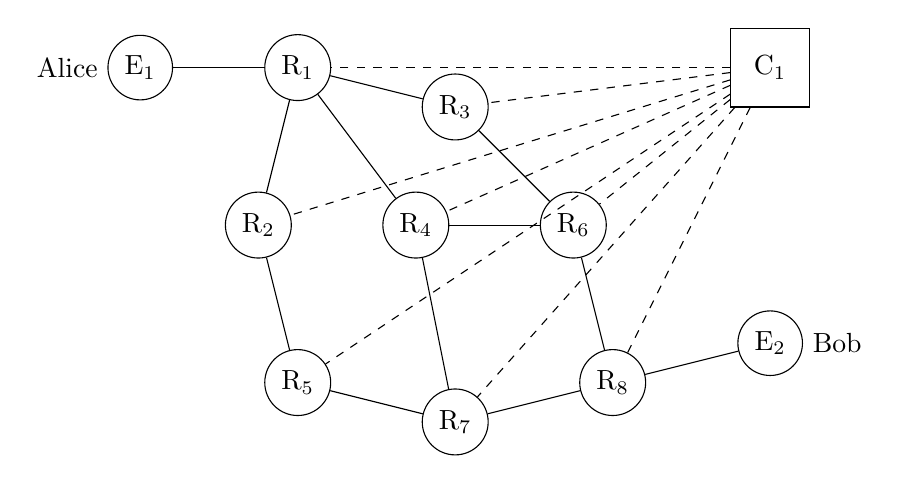
\begin{tikzpicture}
  \tikzstyle{node} = [circle, draw=black]
  \tikzstyle{controller} = [minimum size = 1cm, draw=black]
  \tikzstyle{straight} = [-]
  \tikzstyle{dotted} = [-, style=dashed]

  \node[controller] (c1) at (9,0) {C\textsubscript{1}};
  \node[node] (r1) at (3,0) {R\textsubscript{1}};
  \node[node] (r2) at (2.5,-2) {R\textsubscript{2}};
  \node[node] (r3) at (5,-0.5) {R\textsubscript{3}};
  \node[node] (r4) at (4.5,-2) {R\textsubscript{4}};
  \node[node] (r5) at (3,-4) {R\textsubscript{5}};
  \node[node] (r6) at (6.5,-2) {R\textsubscript{6}};
  \node[node] (r7) at (5,-4.5) {R\textsubscript{7}};
  \node[node] (r8) at (7,-4) {R\textsubscript{8}};
  \node[node, label = {left:Alice}] (e1) at (1,0) {E\textsubscript{1}};
  \node[node, label = {right:Bob}] (e2) at (9,-3.5) {E\textsubscript{2}};

  \draw[dotted] (c1) -- (r1);
  \draw[dotted] (c1) -- (r2);
  \draw[dotted] (c1) -- (r3);
  \draw[dotted] (c1) -- (r4);
  \draw[dotted] (c1) -- (r5);
  \draw[dotted] (c1) -- (r6);
  \draw[dotted] (c1) -- (r7);
  \draw[dotted] (c1) -- (r8);

  \draw[straight] (r1) -- (r2);
  \draw[straight] (r1) -- (r3);
  \draw[straight] (r1) -- (r4);
  \draw[straight] (r2) -- (r5);
  \draw[straight] (r3) -- (r6);
  \draw[straight] (r4) -- (r6);
  \draw[straight] (r4) -- (r7);
  \draw[straight] (r5) -- (r7);
  \draw[straight] (r6) -- (r8);
  \draw[straight] (r7) -- (r8);

  \draw[straight] (e1) -- (r1);
  \draw[straight] (e2) -- (r8);
\end{tikzpicture}
\begin{figure}[H]
  \caption[graph 1 explanation]{The figure shows shows the topology implemented
  by the ``start\_sample\_route.sh''}
  \label{graph explanation}
\end{figure}

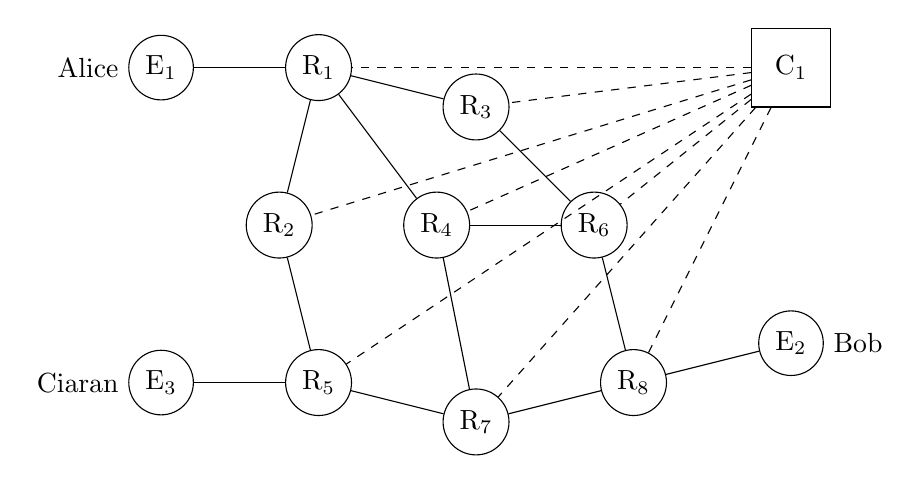
\begin{tikzpicture}
  \tikzstyle{node} = [circle, draw=black]
  \tikzstyle{controller} = [minimum size = 1cm, draw=black]
  \tikzstyle{straight} = [-]
  \tikzstyle{dotted} = [-, style=dashed]

  \node[controller] (c1) at (9,0) {C\textsubscript{1}};
  \node[node] (r1) at (3,0) {R\textsubscript{1}};
  \node[node] (r2) at (2.5,-2) {R\textsubscript{2}};
  \node[node] (r3) at (5,-0.5) {R\textsubscript{3}};
  \node[node] (r4) at (4.5,-2) {R\textsubscript{4}};
  \node[node] (r5) at (3,-4) {R\textsubscript{5}};
  \node[node] (r6) at (6.5,-2) {R\textsubscript{6}};
  \node[node] (r7) at (5,-4.5) {R\textsubscript{7}};
  \node[node] (r8) at (7,-4) {R\textsubscript{8}};
  \node[node, label = {left:Alice}] (e1) at (1,0) {E\textsubscript{1}};
  \node[node, label = {right:Bob}] (e2) at (9,-3.5) {E\textsubscript{2}};
  \node[node, label = {left:Ciaran}] (e3) at (1,-4) {E\textsubscript{3}};

  \draw[dotted] (c1) -- (r1);
  \draw[dotted] (c1) -- (r2);
  \draw[dotted] (c1) -- (r3);
  \draw[dotted] (c1) -- (r4);
  \draw[dotted] (c1) -- (r5);
  \draw[dotted] (c1) -- (r6);
  \draw[dotted] (c1) -- (r7);
  \draw[dotted] (c1) -- (r8);

  \draw[straight] (r1) -- (r2);
  \draw[straight] (r1) -- (r3);
  \draw[straight] (r1) -- (r4);
  \draw[straight] (r2) -- (r5);
  \draw[straight] (r3) -- (r6);
  \draw[straight] (r4) -- (r6);
  \draw[straight] (r4) -- (r7);
  \draw[straight] (r5) -- (r7);
  \draw[straight] (r6) -- (r8);
  \draw[straight] (r7) -- (r8);

  \draw[straight] (e1) -- (r1);
  \draw[straight] (e2) -- (r8);
  \draw[straight] (e3) -- (r5);
\end{tikzpicture}
\begin{figure}[H]
  \caption[graph 2 explanation]{The figure shows shows the topology implemented
  by the ``start\_sample\_route2.sh''}
  \label{graph 2 explanation}
\end{figure}

\subsection{Packet Classes}
The packet classes are encoded using the method ObejectInputStream and
ByteArrayInputStream. This allows us to create a byte array which is then used
to create a DatagramPacket. The abstract class PacketContent and the classes
which inherit it abstract the creation of DatagramPackets. The abstract
methods toByteArray and fromDatagramPacket do the encoding of the
DatagramPacket. Each implementation of the PacketContent class has their own
implementation of the abstract methods toByteArray and fromDatagramPacket. The
abstract PacketContent abstract class and the AckPacketContent class have been
provided to us in the Advanced sample code. I have created other packet classes
which implement the PacketContent abstract class.

\subsubsection{FeatureRequestPacketContent}
This class is used to create a packet which represents a feature request
packet. The feature request packet is sent by the \textbf{Controller} to a
switch upon receiving a Hello packet. The feature request packet does not
contain any data and only contains its type.

\subsubsection{FeatureResultPacketContent}
This class is used to create a packet which represents a feature result packet.
The feature result packet is sent by the \textbf{Switch} to the
\textbf{Controller} in response to a feature request packet from the
\textbf{Controller}. The feature request packet contains information about the
specifications of the \textbf{Switch} such as the number of tables it has and
the size of the buffer. The buffer size and number of tables currently have no
use and is only included as it was a part of the OpenFlow specification. The
feature result packet also contains the \textbf{Switch's} name and its
connections. The switch connections are used when calculating the path to the
specified destination.

\subsubsection{FlowModPacketContent}
This class is used to create a packet which represents a flow mod packet. The
flow mod packet is sent by the \textbf{Controller} to a \textbf{Switch}. The
flow mod packet is used to change a \textbf{Switch's} flow table. The flow mod
packet contains two strings, the destination and the next hop. Upon receiving a
flow mod packet, the \textbf{Switch} update it's flow table with the destination
as the key and the next hop as the value.

\subsubsection{HelloPacketContent}
This class is used to create a packet which represents a hello packet. The hello
packet is sent by both the \textbf{Switch} and \textbf{Controller}. The hello
packet contains the version number. When receiving a hello packet, the lower
version of the protocol is set. In my assignment, the default version number
is set to 1. In my version of OpenFlow, the hello packet is sent first by the
\textbf{Switch} to the \textbf{Controller} upon initialisation. The
\textbf{Controller} then responds with it's own hello packet back to the
\textbf{Switch}. This differs from the actual OpenFlow specification as the
hello packet should be asynchronous.

\subsubsection{PacketInPacketContent}
This class is used to create a packet which represents a packet in packet. The
packet in packet is sent by the \textbf{Switch} to the \textbf{Controller}.
This packet is used to ask the \textbf{Controller} for a flow mod packet. This
packet is sent in the case where a table miss occurs and the switch does not
know where to forward the packet. The packet in packet contains the final
destination of the packet and the switch name. The destination and the switch
name are both keys in the \textbf{Controller's} flow tables.

\subsubsection{PayloadPacketContent}
This class is used to create a packet which represents a payload packet. The
payload packet contains the payload i.e. the string containing the message and
final destination of the packet. This packet is sent by the \textbf{End-Nodes}
as well as the \textbf{Switches}. This packet is the packet which is forwarded
from \textbf{Switch} to \textbf{Switch} and to the final destination
\textbf{End-Node}.

\subsection{Node Classes}
This section includes a description of each of the nodes classes which are
interfaced by the terminal. They represent any type of node in the network.

\includescalefigure{SampleUsage}{Sample usage of protocol}{The figure shows a
  message being sent from Alice to Bob. The hops the packet took and the path
generated by the \textbf{Controller} is shown.}{1}{SampleUsage.png}

\subsubsection{Controller}

\includescalefigure{ControllerRoutePacketForwarding}{Controller doing work}{The
  figure shows the \textbf{Controller} finding a path to the destination
  required and forwarding the appropriate routing tables. The figure shows is
  the result of Alice sending a message to Bob and Bob sending a message to
Ciaran.}{1}{ControllerRoutePacketForwarding.png}

The \textbf{Controller} is used to direct the \textbf{Switches} when they have
no flow table entry for a packet. The \textbf{Controller} sends a flow mod
packet upon receiving a packet in packet. The paths are stored in a hash table.
The key is a string which is the final destination the packet to be forwarded.
The value is another hash table of which the key is the switch. The value is the
next hop the switch has to forward the packet to.

The \textbf{Controller} used to contain a predefined path. However I have since
changed it to use Link State Routing. The \textbf{Controller} uses the Graph
class in order to calculate a path to the destination. If the destination is not
in the hash table, the path is calculated and is then stored into the hash table.
The path is only generated when a \textbf{Switch} requests for the next hop and
the destination is not found in the flow table. If no path is found, the
\textbf{Controller} sends an unknown destination packet to the \textbf{Switch}.

\subsubsection{EndNode}

\includescalefigure{EndNodeMessageSend}{Message send and
  receive}{The figure shows a message being sent and
received}{1}{EndNodeMessageSend.png}

The \textbf{End-Node} is where the user can send and receive messages. The user
is able to choose another \textbf{End-Node} to send the message to. The message
it takes in is of type string and is encapsulated in a payload packet. This
payload packet is sent to a \textbf{Switch} which is then forwarded to another
\textbf{Switch} or to the destination \textbf{End-Node}. When an \textbf{End-Node}
receives a payload packet, the message is printed out to the terminal.

The \textbf{End-Node} implements a command system. This command system contains
the commands ``help'', ``clear'' and ``message send
\textless`message'\textgreater
\textless{}destin-\newline{}ation\textgreater{}''. The ``help'' command is used
to display all the commands available. The ``clear'' command is used to clear the
terminal screen and the ``message send'' command is used to send a string
message to the destination \textbf{End-Node}.

\subsubsection{Node}
This class is an abstract class which all of the \textbf{Node} classes inherit.
This class has been provided to us from the advanced sample code. It has been
modified slightly in the previous assignment, the changes of which is carried
through to this assignment.

\subsubsection{Switch}

\includescalefigure{RouterForward}{Router forwarding messages}{The figure shows
a payload packet forwarded by the \textbf{Switch}, first case where table miss
occurs, second case the packet is forwarded directly to the next hop without
contacting the \textbf{Controller}.}{1}{RouterForward.png}

The \textbf{Switch} class uses a hash table to store the payload packet's next
hop. When the \textbf{Switch} receives a payload packet, the destination is
looked up in the hash table. If the destination in the hash table exists, the
packet is then forwarded to the next hop. If the destination does not exist,
then the \textbf{Switch} sends a packet in packet to the \textbf{Controller}.
A countdown latch is used to wait for a flow mod packet to arrive. Upon the
arrival of a flow mod packet, the payload packet is then forwarded to the
next hop.

A queue called the packet buffer is used to deal with payload packet arrivals.
This allows the payload packets to be handled one at a time.  An infinite loop
is used to process the payload packets in a thread.

\subsection{Path Finding class}
This path finding class is used to implement the link state routing. It
implements the algorithm which computes the path to the destination.

\subsubsection{Graph}
The graph class contains a node class. This node class represents nodes in the
network in a graph. The node class contains the name of the node as well as the
node's adjacent nodes. This abstract data structure is used when calculating the
path to the destination.

All of the nodes are stored in the graph's hash table. The key of the hash
table is a string which is the name of the node. The value of the hash table is
the reference to the node which has that name.

I found it difficult to measure the latency between the connections in Docker
and thus was unable to obtain the weights of the edges in the graph. I used a
breadth first search algorithm instead of Dijkstra's algorithm for this reason.

\subsection{Miscellaneous Classes}
This section contains an explanation of the classes which did not fit into the
other categories.

\subsubsection{Terminal}
The terminal class was provided to us in the sample code. I have slightly
modified the terminal class to have the ability to clear the terminal screen
as well as read a boolean from the user. The boolean function was implemented
using JOptionPane to display a yes or no question. The boolean function however
was not used in this assignment but was used in the first assignment.

\subsubsection{Tokenizer}
The tokenizer class was used to split up the command into tokens and has the
ability to separate messages in quotations. This was created instead of using
the string split function as it allows the message sent to have spaces instead
of being a single word.

\section{Advantages and Disadvantages}
\subsection{Advantages}
\begin{itemize}
  \item{Implements Link State Routing thus allowing any valid switch and
    endpoint connection combinations to be used.}
  \item{Can add more routers to the network on the fly.}
  \item{The network graph can be directed i.e. \textbf{Switches} can have one
    way connections}
  \item{Does not allow the use of multiple \textbf{Controllers}.}
  \item{It is asynchronous due to the use of threads.}
  \item{The implementation is abstracted well using Java's object orientated
    nature and the use of classes.}
\end{itemize}
\subsection{Disadvantages}
\begin{itemize}
  \item{Does not deal with dead routers.}
  \item{Does not deal with invalid or unconnected graphs.}
  \item{Is not an accurate implementation of the OpenFlow specification.}
  \item{Does not implement acknowledgements.}
  \item{Command system may be confusing to the user.}
  \item{Certain network configurations may cause the path to be calculated
    multiple times.}
\end{itemize}

\section{Program Usage}
The following are some instructions to run the project:
\begin{itemize}
  \item{This program was built around the use of Docker.}
  \item{To run the program, the bash script ``start\_sample\_route.sh'',
    ``start\_sam-\\ple\_route2.sh'' or the ``start\_straight\_line.sh'' may be
  used.}
  \item{The script must be run with root due to the nature of Docker and it's
    permissions required to run.}
  \item{The script ``start\_straight\_line.sh'' may take an integer parameter
    to indicate the number of switches between the endpoints e.g. ``sudo
  start\_sta-\\ight\_line.sh 3'' to have three switches between the endpoints.}
\end{itemize}

The program has only been tested on a Linux system and is not guaranteed to run
on a Windows or Mac machine.

\section{Reflection}
This assignment has taught me many things about the OpenFlow software defined
networking standard. Doing this assignment has also taught me more things about
Java threads and concurrent programming as well as Docker and bash scripting. I
also learned a lot about implementing graph algorithms and about graphs in
general.

Overall I am very happy with my implementation of the OpenFlow standard. I would
like to improve on my bash scripting as I feel that the code I produced for the
bash scripts are somewhat hard to read. If I were to complete the project again
I would attempt to implement Dijkstra's algorithm or perhaps even more complex
graph algorithms.

\end{document}
